\documentclass[a4paper,11pt]{article}

\usepackage[british]{babel}
\usepackage{graphicx}

\usepackage{hyperref}
\bibliographystyle{ieeetran}

\title{\textbf{Microcontroller Programming (course 1TE663) \\
    Uppsala University -- Spring 2016 \\
    Project report}}

\author{Per Bergqwist \and Martin Lindström \and Dennis Pietarinen}

\date{\today}

\begin{document}

\maketitle

\tableofcontents

\section{Introduction}
The main goal of this project was to design a protocol to
network a lot of microcontroller using cheap nrf24l01+ modules.  We
decided to develop a self organizing spanning tree mesh network using
a pre-defined node to be sink.  The sink was connected to a pc which
made the mesh network available though a web socket.  The result is
the possibility to make large, cheap, long-range networks which are
accessable though the internet.  Possible use-cases include remote
monitoring and home automation.

\section{Design decisions}
The radiomodules support automatic acknoledgement of packets with
optional retransmissions\cite{nrfDS}. This enabled us to easily make the
communication between two modules reliable. The auto acknoledgement
feature was used in all communication except for new nodes
broadcasting to connect to the network.

The radio modules uses GFSK in the 2.4-2.5125Ghz range with support of
datarates from 250Kbps up to a maximum of 2Mbps. The channels are 1Mhz
wide and there are 126 different channels\cite{nrfDS}. We decided to use the same
frequency for all nodes in the same network to decrease the complexity
of the communication. This makes all communication within the network
interfere but since all communication is acknowledged and checksummed
this won't impact the reliablity of the data.

The radiomodules has internal addressing with addresses consisting of
3-5 bytes. Each module can listen for up to six adresses at the same
time but five of these adresses can only differ in their last
byte\cite{nrfDS}. We decided to let the mcu save the addresses and
routing table and only use two of the addresses in the radio
modules. One for broadcast messages and one for unicast messages
directed towards the specified node. This approach makes it possible
for one node to be parent to a large amount of nodes.

We studied different routing protocols for making a mesh-network,
initally we wanted to have a complete mesh network without a sink but
due to the limited amout of memory availible on the chosen mcu we
decided to go for a spanning tree network instead. We figured that
this would make the routing table use less memory since and be less
complex. Each node keeps a routing table of all nodes locaded below
them in the network and their corresponding parent node. The sink is
the highest parent. This approach uses memory scaling linearly with
the amount of nodes in the network. The nodes only need to know the
route to the nodes located below themselves.

The adress of a node is saved in the microcontrollers EEPROM memory.
This makes it possible to completely shut down a node without it 
needing a new address. This decision makes the network only one 
address per physical node. We thought about assigning addresses based
on the location of the nodes in the network but this increases 
the complexity of the sink node since it would need to keep track of
all active adresses.

\subsection{Hardware}
Each node consists of one atmega328p mcu running from the
internal oscillator at 8Mhz. It's connected to a nrf24l01+ through the
SPI port. The mcu can be connected to an rs232 adapter to enable
debugging messages to a computer. The sink mcu is connected to an
rs232 adapter to interface with the PC. The nodes accept an input
voltage from 2.4v to 3.6v. Since the NRF24l01+ modules can be run at a
minimum of 1.8v we could potentially run the node at 1.8v but this
would require a lower clockfrequency for the mcu\cite{Atmega}. 

We built some battery powered nodes that runs from a li-ion battery
connected to a 3.3v regulator. The regulator is needed to keep the 
input voltage to the radiomodule below 3.6v.



\subsection{Software}
The software on the mcu acts as a big statemachine shown in Figure \ref{fig:state}.

At startup the mcu is in the unconnected stated. In this state the
node is completely unconnected the network. If a node want's to join a
network it needs to send a broadcast which makes it go into the BRD
SENT state. As long as it does not receive any replies the mcu stays
in this state and sends new broadcasts with a fixed interval.

If the node gets a reply from another node it goes into the collecting
parents state. The node stays here and listens to the channel for a
fixed amount of time. If more than one node replies to the broadcast
the node replies to the node with the smallest hop-count and moves to
either the WAIT FOR ADDDRESS state or the CONNECTED STATE. If this
node has received an address before it will keep that address and go
directly to the connect state. Otherwise it will ask the network to
give it a free address and go into the WAIT FOR ADDRESS state.

In the WAIT FOR ADDRESS state the parent node will recognize that the
new nodes does not have an adress and will request a new address from
the sink node. 

The CONNECTED STATE is the default state for an active node. The node
is in receive mode and will listen to the channel constantly. When
it receives a packet it will check if the packet was meant for
itself or if it should re-send it.


\begin{figure}[h!]
  \includegraphics[width=\linewidth]{states}
  \caption{State Diagram}
  \label{fig:state}
\end{figure}

\subsection{Tests}
We measured the current of a non sink node to 13mA at 3.3v. The setup
is shown in figure \ref{fig:Effekt} The current measurement was made from
the output of a 3.3v regulator.  The node was put in a always
listening state. According to the datasheet the radio module should
consume a maximum of 11mA in listening mode.

We did not to any tests for the power consumption in transmitting
mode.

\begin{figure}[h!]
  \includegraphics[width=\linewidth]{EffektMätarSetup}
  \caption{Measuring current with high presision resistor and an oscilloscope}
  \label{fig:Effekt}
\end{figure}

Range test:
We measured the maximum range of one hop to 80m in an outdoor 
enviroment when transmitting at 2.52GHz. 
The maximum indoor range was measured to 70m in an indoor
enviroment transmiting at 2.52GHz. Both tests were done with the nodes within line-of-sight.
 


\section{Interface}
\begin{center}
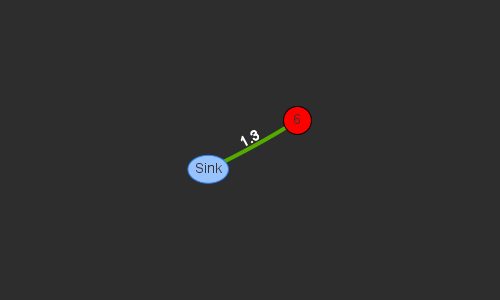
\includegraphics[width=.5\textwidth]{map}
\end{center}

\section{Discussion}
The implementation behaves as expected and has proved to heal itself
if case of disconnection of routing nodes. 

The codes occupies about 8Kb of flash memory and under 700B of
ram. This makes it possible to add more code for gathering sensor data
and possibly interfacing with actuators. 

In it's current state the mcu will have to poll the radio module for
new data but it's possible to make the code interrupt driven.

\section{Future work}
The code could be made interrupt driven by the use of the interrupt 
pin on the radio modules. This would make the nodes faster at reacting
to events from the radio. 

We would like to add some security to the network. Since we are using
wireless signals we are broadcasting all traffic in clear text. As a 
start we could implement an AES engine to provide confidentiality of  
the network traffic. After this is done we might try to add defense against 
replay attacks. 

Another useful feature would be to implement support for sleeping 
nodes. These nodes would only be powered on at certain intervals to
save energy. The idea is to have these nodes at the edge of the 
network so they do not have to route any traffic. As the code works
now these nodes will have to register themselves on the network
everytime they wake up. 

The internet interface would be better if the user could send commands
into the network. At the current state we can only get information out
from the network but send any commands.

\begin{thebibliography}{2}

\bibitem{nrfDS}
  Nordic Semiconductors. "\emph{nRF24L01 Product specification}". sida [Online]. Available: \url{http://www.nordicsemi.com/eng/content/download/2730/34105/file/nRF24L01_Product_Specification_v2_0.pdf} [Accessed: Mar. 09, 2016]

\bibitem{Atmega}
  Atmel. "\emph{ATMEL 8-BIT MICROCONTROLLER}". sida [Online]. Available: \url{http://www.nordicsemi.com/eng/content/download/2730/34105/file/nRF24L01_Product_Specification_v2_0.pdf} [Accessed: Mar. 09, 2016]

\end{thebibliography}
\end{document}


